\chapter{Descubrimiento supervisado de procesos}
\label{chap:3}

En este capítulo, nos centraremos en el área de la minería de procesos que refiere
al descubrimiento de procesos. Como vimos, el descubrimiento de procesos busca un modelo 
que represente el funcionamiento de un cierto sistema a partir de un log del mismo.
Para ello, revisamos el algoritmo de descubrimiento introducido en~\cite{LeonCB15},
el cual consiste en una extensión del algoritmo en~\cite{CarmonaC14} que permite 
introducir información negativa al proceso de búsqueda. De este análisis se observan 
ciertas limitaciones que posee este enfoque, por lo cual planteamos un nuevo 
algoritmo de descubrimiento como una extensión al proceso en~\cite{LeonCB15} mediante 
la que buscamos salvar estos inconvenientes con el fin de obtener, de manera automática, 
un modelo que sea a la vez adecuado, preciso, general y simple.

Se detallará el algoritmo de descubrimiento propuesto y se mostrará además,
que la técnica de simplificación introducida es independiente del proceso de descubrimiento
y puede ser utilizado para simplificar los modelos obtenidos por otras técnicas.

\section{Algoritmo de descubrimiento}
\label{sec:3.algodisco}

Según lo visto en la~\autoref{sec:2.discovery discovery}, el descubrimiento de procesos
refiere a la técnica mediante la cual, partiendo del log de un sistema, se busca
un modelo que lo represente.
Para este fin, existen diferentes metodologías~\cite{CarmonaC14,LeonCB15,MedeirosAW03,AalstWM04}.
En este trabajo, se introduce una extensión del algoritmo presentado en~\cite{LeonCB15} (el cual a
su vez consiste en una extensión de~\cite{CarmonaC14}). Este algoritmo posee algunas falencias
que se detallan a continuación.

El primer inconveniente, proveniente del enfoque utilizado en~\cite{CarmonaC14}, 
surge del crecimiento exponencial de su complejidad con respecto al número de actividades 
en un log: se introduce una estrategia del tipo \dquote{divide y vencerás}, 
utilizando proyección -\textit{projection}- así como el concepto de muestreo -\textit{sampling}-.
Las técnicas de muestreo y proyección, conforman una solución satisfactoria al problema del
crecimiento exponencial, pero al mismo tiempo, la calidad de las métricas referentes a 
precisión y simplicidad suelen ser degradadas considerablemente generando un modelo complejo
que admite demasiados comportamientos además de los observados en el log, 
i.e. se obtiene un modelo \textit{overfitting}.

\begin{remark}[Projection]
    \textit{Projection} hace referencia al principal método utilizado para aliviar la carga
    computacional inherente al algoritmo de descubrimiento utilizado, cuya complejidad
    crece exponencialmente en relación a los puntos del conjunto de vectores Parikh de un cierto
    log. Projection es un método del tipo divide y vencerás que consta de tres partes. 
    La primera se ocupa de agrupar los eventos del log en grupos -\textit{clusters}-
    para los cuales existe un alto grado de correlación. 
    Luego se resuelve el problema de manera aislada para cada uno de los grupos.
    Por último, se buscan relaciones entre los diferentes grupos de manera de 
    conectar las diferentes soluciones de los subproblemas en lo que será
    el modelo final del problema.
\end{remark}

\begin{remark}[Sampling]
    \textit{Sampling} corresponde a una técnica utilizada para hacer factible utilizar
    logs de gran tamaño, lo cual es usual.
    Obtener la cápsula convexa posee un alto costo computacional, por lo que, sí el log utilizado
    como argumento es de gran tamaño, lo hace impracticable.
    Mediante sampling lo que se hace es seleccionar de manera aleatoria un subconjunto de los
    puntos del conjunto de vectores Parikh correspondiente al log como entrada para calcular y 
    luego se filtran aquellos resultado obtenidos, eliminando aquellos que no admitan alguno 
    de los puntos iniciales.
\end{remark}

\begin{example}
    Sea el log $\pmlog=\{ ac, abac, abab \}$ cuyo vector de Parikh es 
    $\parikh{\pmlog}=\{ (0,0,0),(1,0,0), (1,0,1),(1,1,0), (2,1,0), (2,1,1),(2,2,0) \}$ (asumiendo el orden $(a,b,c)$).
    Si se proyecta sobre las actividades $\{a,b\}$ y se utiliza una muestra con los puntos
    $\{(1,0,1),(1,1,0),(2,1,1),(2,2,0)\}$, el conjunto de puntos proyectados es
    $\{ (1,0), (1,1), (2,1), (2,2) \}$. 
    Así, utilizando las técnicas en~\cite{CarmonaC14}, se obtendrá la inecuación
    \mbox{$a \ge b$}.
    
    Puede observarse que esto representa una subestimación del modelo ideal (si se consideran
    todos los puntos del log), cuya $H$-representación corresponde a la inecuación $a \ge b + c$.
\end{example}

La segunda limitación surge de la metodología utilizada para computar el poliedro que contiene los 
puntos en el conjunto de vectores de Parikh. Debido a la metodología utilizada, se obtiene un 
modelo complejo del sistema. Existe en~\cite{CarmonaC14} un post procesamiento de simplificación, pero este es
realizado de manera heurística y manual, seleccionando un subconjunto de las restricciones que conforman la
$H$-representación del poliedro computado. Solo se utilizan las restricciones con coeficientes \dquote{simples}, 
eliminando el resto del modelo. 
Esta elección esta basada en la presunción de que, en la vida real, los procesos son definidos de manera
que sean \textit{simples} y más especialmente en el campo de la gestión de procesos de negocio. Esta presunción,
aunque no es necesariamente desacertada, generaliza demasiado el modelo, convirtiéndolo en un modelo
impreciso.

Por su parte, en~\cite{LeonCB15} se propone un método supervisado para la simplificación del modelo que 
introduce el manejo de información negativa.
De manera iterativa, se consideran cada uno de los hiperplanos que conforman la $H$-representación del poliedro
y se intenta desplazar y rotar el mismo para obtener un modelo más simple.
Para evitar degradar el sistema, se limitan las simplificaciones a realizar sobre cada inecuación
de manera que cada punto aceptado inicialmente siga siendo aceptado y se restringe también
de manera que ningún punto prohibido sea aceptado.

El inconveniente con este enfoque es que trata los hiperplanos de manera aislada; cada inecuación
simplificada debe incluir, al menos, las mismas soluciones que la original (para evitar un modelo no adecuado) y no
debe incluir ningún punto negativo. Sin embargo, dado que el comportamiento del sistema no es definido por los 
semiespacios aislados sino por la intersección de todos ellos, es el modelo quien debe admitir los puntos del log,
y restringir los puntos prohibidos y no un semiespacio particular.

\begin{example}
    \label{ex:prob_gen}
    En la~\autoref{fig:glob_encoding}, se muestra un poliedro inicial~\autoref{sfig:glob_encoding.1} 
    y un punto $(9,4)$ que pertenece al semiespacio definido por el plano $p$ pero no al poliedro.

    \begin{figure}[H]
      \centering
      \subbottom[\label{sfig:glob_encoding.1}]{%
        \scaledinput{0.40}{img/ineq1}}
      \hfill
      \subbottom[\label{sfig:glob_encoding.2}]{%
        \scaledinput{0.40}{img/ineq2}}
      \caption{Simplificación individual vs. simplificación estructural.}
      \label{fig:glob_encoding}
    \end{figure}

    Si se aplica la técnica propuesta en~\cite{LeonCB15} a este plano de manera aislada,
    no se obtendrá nunca el poliedro $p'$ en la~\autoref{sfig:glob_encoding.2} ya que
    $p'$ no admite como solución al punto $(9,4)$. 
    Sin embargo, es claro que el punto $(9,4)$ no pertenece al poliedro~\autoref{sfig:glob_encoding.2}.
\end{example}

\subsection{Etapas del procedimiento propuesto}
\label{sec:3.algodisco stages}

El procedimiento propuesto para descubrimiento y simplificación de procesos se ilustra en la~\autoref{fig:flow}.
En la parte superior, dentro del marco negro, se representa el enfoque utilizado en~\cite{CarmonaC14} 
mediante el cual se obtiene un modelo sin utilizar trazas negativas; corresponde a la interpretación
de un log como un conjunto de vectores Parikh, luego la obtención de un poliedro y por ultimó a la 
transformación a una red de Petri según se detalló en la~\autoref{sec:2.discovery}.

\begin{figure}[H]
    \begin{center}
%\scalebox{1}{\input{img/flow.pdf_t}}
    \scalebox{.5}{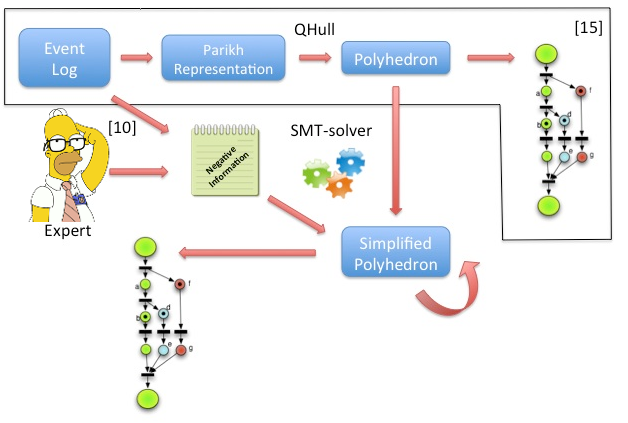
\includegraphics{img/approach_homero}}
    %\scalebox{.6}{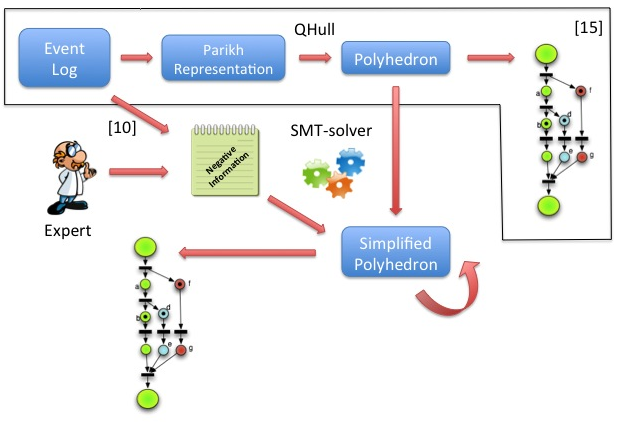
\includegraphics{img/bak_approach}}
    \caption{Comparativa de los diferentes enfoques de descubrimiento de procesos.}
    \label{fig:flow}
    \end{center}
\end{figure}

Por otro lado, en la sección inferior de la~\autoref{fig:flow}, se representa a modo de introducción,
cómo el uso de información negativa proveniente de diferentes medios, se utiliza para simplificar 
el modelo obtenido con el costo de incluir nuevos puntos al modelo final.
Los detalles de este enfoque se precisan a continuación.

\begin{algorithm}[H]
\caption{Descubrimiento de procesos supervisado}
  \begin{algorithmic}[1]
      \Require trazas positivas $\pmlog^+$ y trazas negativas $\pmlog_-$
      \Ensure una red de Petri $N$ donde $\forall \sigma \in \pmlog^+: \sigma \in L(N)$ y $\forall \sigma \in \pmlog_-: \sigma \not \in L(N)$
      \vspace{1pt}
      \Procedure{DISCOVER}{$\pmlog^+, \pmlog_-$}
      \State $pp, np \leftarrow \emptyset$ \label{algo:line1}
      \For{$\sigma_p \in \pmlog^+$}
        \For{$\sigma$ prefix of $\sigma_p$}
          \State add $\widehat\sigma$ to $pp$
       \EndFor
     \EndFor
      \For{$\sigma_n \in \pmlog_-$}
        \State add $\widehat\sigma_n$ to $np$
      \EndFor \label{algo:line2}
      \State $H$ = \textsc{ConvexHull}($pp$) \label{algo:lineqhull}
      \State $H_{smt}$ = \textsc{Shift\&Rotate}($H, np$)
      \State $H'$ = \textsc{Removal}($H_{smt}, np$)
      \State $N$ = \textsc{Hull2Net}($H'$)
      \State \Return N
      \EndProcedure
  \end{algorithmic}
  \label{algo}
\end{algorithm}

El~\autoref{algo} describe paso a paso el enfoque propuesto utilizando pseudocódigo. Un conjunto de trazas 
positivas y un conjunto de trazas negativas conforman la entrada 
(respectivamente \dquote{log de eventos} e \dquote{información negativa} en la~\autoref{fig:flow}). 
En las líneas~\ref{algo:line1}-\ref{algo:line2} se calculan todos los puntos positivos $pp$ para
cada prefijo de una traza positiva en $\pmlogp$ y los puntos negativos $np$ para las trazas en $\pmlogn$\footnotemark[1].
Luego, se calcula un poliedro que contenga el conjunto de puntos $pp$ mediante \textsc{ConvexHull} utilizando 
métodos de programación lineal para obtener la cápsula convexa, e.g. \qhulltool~\cite{Barber96}.

El poliedro que se obtiene es luego simplificado de manera supervisada mediante la función 
\textsc{Shift\&Rotate} utilizando SMT-solvers. El resultado que se obtiene de un SMT-solver es 
una instancia de SMT, la cual no necesariamente provee la solución óptima (pueden existir múltiples soluciones), 
por lo que se utiliza un proceso de refinamiento iterativo para conseguir el óptimo.

La función \textsc{Removal} corresponde a la optimización del procedimiento de eliminación presentado en~\cite{LeonCB15}.
En este punto, se considera, de existir, la información negativa $np$, eliminando únicamente aquellos hiperplanos
que no agreguen ninguno de los puntos de $np$ al modelo.

Por último, el conjunto de semiespacios es transformado en una red de Petri mediante \textsc{Hull2Net} utilizando
la dualidad que existe entre los poliedros y las ecuaciones de marking de una red de Petri
presentada en la~\autoref{sec:2.discovery discovery}.
Cabe destacar que este procedimiento es uno de los pocos que permite obtener todo el conjunto de redes de Petri P/T puras,
i.e. redes de Petri con con fichas y arcos ponderados de manera arbitraria.

Del hecho de que el resultado de \textsc{ConvexHull} puede depender de las técnicas de muestreo y proyección y del
hecho que que \textsc{Shift\&Rotate} está representado como una instancia de SMT (la cual puede poseer múltiples soluciones
y la devuelta depende de la implementación del solver) el algoritmo~\autoref{algo} es no determinista, i.e. dados
los mismos logs positivo y negativo de entrada se pueden obtener diferentes resultados.

\footnotetext[1]{Nótese que en el caso de las trazas negativas, se utilizan únicamente los puntos correspondientes
    a cada traza completa y no a todos sus prefijos. Esto se debe a que para la mayor parte de las trazas negativas 
    el prefijo es compartido con alguna traza positiva por lo que no deben evitarse.}
    
\section{Generalización y simplificación}
\label{sec:3.gensimp}

En la~\autoref{sec:2.discovery} se explica cómo partiendo de un conjunto de logs de un sistema, se puede
buscar un poliedro convexo que contenga al conjunto de vectores Parikh y luego considerar la $H$-representación para
obtener una red de Petri que modele el sistema que generó el log; estos pasos corresponden
a las líneas~\ref{algo:line1}-\ref{algo:lineqhull} de~\autoref{algo}.
Sin embargo, la estructura de esta red suele ser excesivamente compleja debido a que se utilizan 
algoritmos de programación lineal que no calculan un poliedro arbitrario que contenga los puntos,
sino que calculan la cápsula convexa. Aunque en primer instancia puede parecer algo positivo, la restricción
de minimalidad impuesta genera modelos demasiado complejos, alejados del proceso real, lo que
implica que el modelo pierda utilidad. Por este motivo, luego de obtener el modelo, se realiza un post
procesamiento para simplificar el poliedro y por ende el modelo.

\begin{example} 
    \label{ex:polyhedra}
    En la~\autoref{sfig:simp.1} se muestra un poliedro (el área gris claro) cuya $H$-representación viene
    dada por la intersección de los semiespacios definidos por $\{p_0,p_1\}$ y algunas de las caminatas generadas por las trazas.
    Mediante el proceso de generalización, puede obtenerse el poliedro definido 
    mediante la intersección de los semiespacios $\{p_0,p_2\}$ (la unión de las áreas gris clara y gris oscura), 
    i.e. un poliedro cuyo $Z$-poliedro contiene más puntos.
    Los puntos marcados mediante $\bullet$ no son solución de $\{p_0,p_1\}$ pero si lo son de $\{p_0,p_2\}$.
    La~\autoref{sfig:simp.2} y la~\autoref{sfig:simp.3} muestran las redes de Petri inferidas por cada uno 
    de los poliedros. 

    La secuencia de eventos $xxxyxxx$ (asumiendo la representación de los eventos siguiendo la usual de los 
    ejes cartesianos) es una traza de la red en la~\autoref{sfig:simp.3} pero no de la red en la~\autoref{sfig:simp.2}.
    Esto se ve representado en la~\autoref{sfig:simp.1} mediante el punto $(6,1)$, el cual es solución de $\{p_0,p_2\}$,
    pero no es solución de $\{p_0,p_1\}$.
\end{example}

Simplificar un modelo, en la representación utilizada, puede lograrse al remover 
de la $H$-representación del poliedro algunos semiespacios. Debido a que cada inecuación
define un place en la red, al eliminarlas, se reduce el número de places en la red y por lo tanto,
se obtiene un modelo más simple. 
%Para seleccionar los semiespacios a eliminar, puede utilizarse
%información experta (si se cuenta con ella) para detectar aquellas situaciones donde el modelo
%presentado es por demás restrictivo y puede relajarse.
La propuesta de este trabajo es la de \dquote{desplazar} -\textit{shift}- y \dquote{rotar} 
-\textit{rotate}- el poliedro obtenido para obtener restricciones más simples, 
preservando lo más posible el comportamiento original. Este procedimiento
de generalización se realiza de manera automática mediante el uso de SMT-solvers, 
verificando que no se introducen comportamientos prohibidos en el proceso.
Luego de estas simplificaciones, la red de Petri relacionada al poliedro acepta
una cantidad de trazas mayor, generalizando el comportamiento subyacente. 
Como se vio en la~\autoref{sec:3.algodisco}, el algoritmo propuesto en~\cite{LeonCB15}
propone un procedimiento supervisado de simplificación, pero es demasiado restrictivo
debido a su naturaleza iterativa de procesamiento (\autoref{ex:prob_gen}).

La propuesta de esta tesina para mejorar el enfoque anterior, consiste en considerar
en el algoritmo de simplificación, la matriz de incidencia y el marking inicial como
una unidad en lugar de intentar simplificar las inecuaciones una a una.
Dado un sistema de la forma:

\begin{center}
    $\begin{array}{rcccccccl}
        \alpha_{1,0} & + & \alpha_{1,1} \cdot x_1 & + & \dots & + & \alpha_{1,n} \cdot x_n & \ge & 0 \\
        \alpha_{2,0} & + & \alpha_{2,1} \cdot x_1 & + & \dots & + & \alpha_{2,n} \cdot x_n & \ge & 0 \\
            \vdots & & & & & & \vdots \\
        \alpha_{m,0} & + & \alpha_{m,1} \cdot x_1 & + & \dots & + & \alpha_{m,n} \cdot x_n & \ge & 0
    \end{array}$
\end{center}

se buscan nuevos coeficientes $\beta_{1,0},\beta_{1,1}, \dots, \beta_{m,n}$ tal que:

\bequationl{enc1} \tag{NZ}
    \sum\limits_{i,j=1}^{m,n} \beta_{i,j} > 0 \text{ y } \sum\limits_{i=1}^{m} \beta_{i,0} > 0
\eequation

Para cada $0 \leq i \leq m$ y $1 \leq j \leq n$,

\bequationl{enc2} \tag{MIN}
    \rvert \beta_{i,j} \lvert\ \leq\ \rvert \alpha_{i,j} \lvert
\eequation

y para todo $x_j \ge 0$ con $1 \leq j \leq n$,

\bequationl{enc3}\tag{PC}
    \bigwedge\limits_{i=1}^m (\alpha_{i,0} + \sum\limits_{j=1}^n \alpha_{i,j} \cdot x_j )\ge 0 \ \Rightarrow\ \bigwedge\limits_{i=1}^m (\beta_{i,0} + \sum\limits_{j=1}^n \beta_{i,j} \cdot x_j) \ge 0
\eequation

Coloquialmente, \eqref{eq:enc1} especifica que al menos uno de los coeficientes debe ser no nulo,
para eliminar las soluciones triviales y que el marking inicial conste, cuanto menos, de un token.

El significado de \eqref{eq:enc2} por su parte, indica que la nueva matriz debe ser, al menos tan 
simple como la original.

Por último, cada solución del sistema inicial (como un todo) debe ser también una solución del nuevo
sistema para asegurar que mantenemos un modelo adecuado, esto se refleja en~\eqref{eq:enc3}.

Para obtener la $H$-representación de un poliedro que implique una representación más simple y general de una red de Petri, 
las condiciones \eqref{eq:enc1}, \eqref{eq:enc2} y \eqref{eq:enc3} pueden ser codificadas utilizando 
satisfabilidad módulo teorías. 

\begin{example}
Para la matriz de incidencia de~\autoref{sfig:simp.2}, la codificación como SMT resulta

%\todo{Esto no se puede ordenar más lindo? No me gusta...}
$$\begin{array}{l}
{(\beta_{1,1} + \beta_{1,2} + \beta_{2,1} + \beta_{2,2} > 0)} \land
{(\beta_{1,0} \geq 0)} \land
{(\beta_{2,0} \geq 0)} \land \\ \\
{(\lvert \beta_{1,1} \rvert \leq 2)} \land
{(\lvert \beta_{1,2} \rvert \leq 3)} \land
{(\lvert \beta_{2,1} \rvert \leq 1)} \land
{(\lvert \beta_{2,2} \rvert \leq 1)} \land \\ \\
{\forall \widehat\sigma(x), \widehat\sigma(y) : (6 - 2 \cdot \widehat\sigma(x) + 3 \cdot \widehat\sigma(y) \ge 0 \land 1 + \widehat\sigma(x) - \widehat\sigma(y) \ge 0)} \\ \\
\Rightarrow (\beta_{1,0} + \beta_{1,1} \cdot \widehat\sigma(x) + \beta_{1,2 }\cdot  \widehat\sigma(y) \ge 0 \land \beta_{2,0} + \beta_{2,1} \cdot \widehat\sigma(x) + \beta_{2,2} \cdot  \widehat\sigma(y) \ge 0)
\end{array}$$

para esta codificación, se obtiene automáticamente la siguiente solución (mediante el uso de los SMT-Solvers)

$$\beta_{1,0}=6,\beta_{1,1}=-1,\beta_{1,2}=2, \beta_{2,0}=1,\beta_{2,1}=1,\beta_{2,2}=-1$$

correspondiente al marking de la red en la~\autoref{sfig:simp.3}.
Se puede ver que el método propuesto no sacrifica lo adecuado del modelo, ya que el $Z$-poliedro obtenido
contiene al original.
\end{example}

\begin{theorem}
    \label{theo:fit}
    Sea $\pmlog$ un log, $N$ un modelo adecuado de $\pmlog$ y $N'$ el modelo obtenido según el método propuesto,
    entonces $N'$ es adecuado para $\pmlog$.
\end{theorem}

\begin{proof}
    Sean $$\mathcal{P} = \bigwedge\limits_{i=1}^m (\alpha_{i,0} + \sum\limits_{j=1}^n \alpha_{i,j} \cdot x_j )\ge 0$$ y
    $$\mathcal{P}' = \bigwedge\limits_{i=1}^m (\beta_{i,0} + \sum\limits_{j=1}^n \beta_{i,j} \cdot x_j )\ge 0$$ los poliedros
    obtenidos de las ecuaciones de marking de $N$ y $N'$ respectivamente. Dado que $N$ es adecuado para $\pmlog$ por hipótesis, 
    todos los puntos correspondientes al conjunto de vectores Parikh de $\pmlog$ son solución de $\mathcal{P}$.
    A partir de lo anterior y de~\eqref{eq:enc3}, todos los puntos son solución de $\mathcal{P}'$.
    Por lo tanto, todas las trazas de $\pmlog$ son ejecutables en $N'$, i.e. $N'$ es adecuado para $\pmlog$.
\end{proof}

\subsection{Uso de información negativa}
\label{sec:3.gensimp negative}

El proceso de generalización y simplificación propuesto en la~\autoref{sec:3.gensimp} introduce nuevos puntos al modelo, 
los cuales generan nuevos comportamientos del sistema representado. Si se cuenta con un log negativo
puede considerarse esta información para asistir al procedimiento y evitar la degradación
de la solución.

Para utilizar un log negativo, se procede a considerar la representación como vectores Parihk de las trazas negativas.
Luego se consideran estos puntos como restricciones al aplicar la simplificación \textsc{Shift\&Rotate}; es decir, se debe 
verificar que las transformaciones realizadas al poliedro no conviertan a estos puntos en puntos válidos.

Como se vio en la~\autoref{sec:3.algodisco}, el enfoque presentado en~\cite{LeonCB15},
introduce las trazas negativas en el algoritmo de simplificación.
En cada procesamiento aislado de los hiperplanos, se limitan las simplificaciones 
aplicadas a cada uno de manera que el hiperespacio no admita \emph{ningún} punto negativo.
Esta estrategia posee un problema análogo al considerado con información únicamente positiva; en este caso
un hiperespacio puede contener un punto negativo siempre que exista otro hiperespacio
que no lo admita.

\begin{example}
    En la~\autoref{fig:glob_encoding}, sea~\autoref{sfig:glob_encoding.1} el poliedro
    a simplificar y sea $(8,4)$ un punto prohibido, que correctamente no se encuentra entre los
    punto interiores al poliedro.
    
    La técnica propuesta en~\cite{LeonCB15}, aplicada al plano $p$ de manera aislada, 
    no obtendrá nunca el poliedro en la~\autoref{sfig:glob_encoding.2} ya que
    el semiespacio inducido por $p'$ admite como solución el punto negativo. Sin embargo, es claro que el
    el punto $(8,4)$ no pertenece al poliedro~\autoref{sfig:glob_encoding.2}.
\end{example}

De manera similar a lo realizado al considerar las trazas positivas, el algoritmo de simplificación
puede ser optimizado si se consideran el conjunto completo de los hiperespacios en lugar de un
procesamiento aislado. 
Para evitar los comportamientos prohibidos, se utilizará la siguiente condición para cada 
uno de los puntos negativos $(k_1,\dots,k_n)$,

\bequationl{enc4} 
    \tag{NP}
    \begin{array}{rccccl}
        \bigvee\limits_{i=1}^m(\beta_{i,0} & + &\sum\limits_{j=1}^n \beta_{i,j} \cdot k_j) &< &0
    \end{array}
\eequation

Mediante esta representación, se fuerza que, para cada punto negativo,
al menos una de las inecuaciones no se satisfaga.

Si no se cuenta con información negativa, la restricción \eqref{eq:enc1} es necesaria para evitar 
la solución trivial (i.e. remover todos los hiperplanos), esto no ocurre en el caso en el que se conocen
comportamientos prohibidos; la solución trivial admitiría cualquier comportamiento negativo, por 
lo que podemos prescindir de \eqref{eq:enc1}.

\begin{example} 
    \label{ex:polyhedra_part2}
    Retomando el~\autoref{ex:polyhedra}, si se desea generalizar y simplificar el modelo sin admitir el punto $(6,1)$,
    correspondiente al comportamiento $xxxyxxx$, utilizando la nueva representación, se debe agregar la restricción
    
    \bequation
        \begin{array}{lcr}
            (\beta_{1,0} + \beta_{1,1} \cdot 6 + \beta_{1,2} \cdot 1 < 0) &\lor& (\beta_{2,0} + \beta_{2,1} \cdot 6 + \beta_{2,2} \cdot 1 < 0)
        \end{array}
    \eequation

    la cual elimina $\beta_{1,0}=6,\beta_{1,1}=-1,\beta_{1,2}=2, \beta_{2,0}=1,\beta_{2,1}=1,\beta_{2,2}=-1$ 
    como una solución del sistema.

    Utilizar este algoritmo con información negativa, remplaza el primer semiespacio por 
    $5 -2 \cdot \widehat\sigma(x) +2 \cdot \widehat\sigma(y) \ge 0$ y mantiene el segundo.

    La red simplificada que se obtiene corresponde a la que se ve en la~\autoref{fig:neg}, donde
    se observa que no acepta $xxxyxxx$ como traza.

    \begin{figure}[H]
        \centering
        \begin{tikzpicture}

  \node[transition] (x) at (-.75,-1) {$x$};
  \node[transition] (y) at (.75,-1) {$y$};
  \node[tplace,label=above:$p_3$] (p1) at (0,0) {};
  \node[tplace,label=below:$p_0$] (p2) at (0,-2) {};
      
  \node[] (t) at (p1) {5};
  \node[] (t) at (p2) {1};
    
  \draw[style={->,>=triangle 45}] (p1) edge node[above left]{2} (x);
  \draw[style={->,>=triangle 45}] (x) to (p2);    
  \draw[style={->,>=triangle 45}] (p2) to (y);      
  \draw[style={->,>=triangle 45}] (y) edge node[above right]{2} (p1);

  \node[] (null) at (0,-3) {};
    
\end{tikzpicture}
        \caption{Red de Petri utilizando información negativa.}
        \label{fig:neg}
    \end{figure}

\end{example}

\subsection{Eliminación automática de semiespacios}
\label{sec:3.removal}

El último aspecto del proceso de simplificación y generalización,
consiste en la eliminación automática  de semiespacios,
realizada mediante el procedimiento \textsc{Removal}.
Este procedimiento toma como argumento un poliedro y un conjunto de puntos
negativos e itera sobre los hiperplanos que definen el poliedro,
verificando si eliminar el hiperplano convierte en alcanzable algún punto negativo.
Si este no es el caso, la restricción puede ser eliminada sin incorporar
ningún comportamiento prohibido al modelo del sistema. El procedimiento \textsc{Removal}
se encuentra detallado en el~\autoref{algo:rem}. El proceso $\textsc{SomeInside}(H \setminus h, np)$
retorna \textit{true} si eliminar $h$ tiene como consecuencia que algún punto en $np$
sea una solución de $H \setminus {h}$.

\begin{algorithm}[h]
\caption{Eliminación automática de semiespacios}
    \begin{algorithmic}[1]
        \Procedure{Removal}{$H, np$}
            \For{$h \in semiespacios(H)$}
                \If{$\neg \textsc{SomeInside}(H \setminus h, np)$}
                    \State eliminar $h$ de $H$
                \EndIf
            \EndFor
            \State \Return $H$
        \EndProcedure
    \end{algorithmic}
    \label{algo:rem}
\end{algorithm}

El resultado de este procedimiento depende de la calidad de la información negativa:
un mal conjunto de trazas prohibidas puede permitir remover demasiados semiespacios,
deteriorando la precisión de la red de Petri final. Como podrá verse en los experimentos,
las trazas que se obtienen en~\cite{BrouckeWVB14} permiten remover semiespacios sin 
impactar en gran medida la calidad de las métricas de la red.

\subsection{Conceptos de simplicidad y complejidad}
\label{sec:3.complexity}

Existen diferentes conceptos de simplicidad referidos a las redes de Petri~\cite{Lassen08,Mendling2007}. 
La mayor parte se centran en la simpleza visual del modelo final. Sin embargo, estás métricas usualmente 
son definidas en una clase de redes de Petri más restrictiva, donde el principal objetivo radica en la 
representación de flujos de trabajo. Por su parte, las redes utilizadas en este trabajo resultan más generales
y permiten representar conceptos como recursos y costos. Por este motivo, se utiliza una definición más adecuada
de simplicidad para medir la eficiencia buscada.

La idea principal radica en minimizar los coeficientes correspondientes a la matriz de incidencia de la red.
La complejidad de una cierta red resulta de la suma de los valores absolutos de los tokens iniciales, 
los tokens consumidos y los tokens producidos por cada transición.

\begin{definition}
    \label{def:complex}
    (Complejidad estructural) Dada una red de Petri cuyo marking inicial es $(\alpha_{1,0}, \dots, \alpha_{m,0})$ y su matriz de incidencia
    \begin{equation*}
        \left(\begin{array}{ccc} \alpha_{1,1} & \dots & \alpha_{1,n} \\  \vdots & & \vdots \\ \alpha_{m,1} & \dots & \alpha_{m,n}\end{array} \right)
    \end{equation*}

    su \textit{complejidad estructural} viene dada por 
    \bequation
        \sum\limits_{i=1}^m (\lvert \alpha_{i,0} \rvert + \sum\limits_{j=1}^n \lvert \alpha_{i,j} \rvert).
    \eequation
\end{definition}

Luego, la \emph{simplicidad} de una red de Petri es inversamente proporcional a su complejidad estructural. Es decir
que una cierto modelo $N'$ es considerado \textit{más simple} que un modelo $N$ siempre que la red de Petri 
que representa a $N'$ posea una complejidad estructural menor a la red que representa al modelo $N$.

\begin{example}
    La complejidad de los poliedros~\autoref{sfig:simp.1} y~\autoref{sfig:simp.2} siguiendo 
    la~\autoref{def:complex} es 14 y 12 respectivamente.
    Por lo tanto, la red correspondiente a~\autoref{sfig:simp.2} es considerada más simple.
\end{example}

\begin{definition}
    \label{def:effectiveness}
    (Eficiencia porcentual) Dada una red de Petri $N$ cuya complejidad según~\autoref{def:complex} es $c_i$ y sea
    $N'$ la red de Petri obtenida luego de aplicar el método de simplificación presentado cuya complejidad
    es $c_f$, la \textit{eficiencia porcentual} es
    $$\xi = (100 - 100 \times ( c_f / c_i )) \%$$
\end{definition}

\begin{example}
    La~\autoref{fig:mot} muestra el resultado de aplicar el método presentado; la red~\autoref{sfig:mot.1} posee
    complejidad $c_1 = (6 + 2 + 3) + (1 + 1 + 1) + (2 + 1) + (1+1+1) + (3+1) + 1 = 25$ mientras que 
    la red~\autoref{sfig:mot.2}, obtenida luego de aplicar el algoritmo presentado, posee complejidad 
    $c_2 = (2+1+1) + (1+1+1) + (2+1) + (1+1) + (3+1) + 1 = 17$. En este ejemplo, la eficiencia porcentual del
    procedimiento es $\xi = 100 - 100 \times (c_2 / c_1) = 32\%$.
\end{example}

Es importante destacar que existen casos donde la noción de complejidad introducida coincide con las utilizadas
en~\cite{Lassen08,Mendling2007} en el sentido de indicar qué red es más simple, debido a que, remover un hiperplano,
es equivalente a simplificar todos sus coeficientes hasta cero. Sin embargo, este no es siempre el caso.
Siguiendo la definición aquí propuesta, una red que contenga
dos places y coeficientes pequeños (en valor absoluto) es más simple que una red que contenga un único place con 
coeficientes altos lo cual contradice las métricas que se ocupan en la simplicidad visual (e.g. contar la cantidad
de places de una red).

\subsection{Simplificación de modelos arbitrarios}
\label{sec:3.simplification}

Es importante observar que las técnicas presentadas en este capítulo son independientes al algoritmo de 
descubrimiento presentado en~\cite{CarmonaC14} y pueden ser aplicadas sobre cualquier
red de Petri que satisfaga las hipótesis, i.e. cualquier red de Petri pura, sin transiciones silenciosas y sin
dos transiciones representando una misma acción. 

En la~\autoref{sec:2.discovery}, se explica la correspondencia entre un poliedro y una de de Petri mediante
la $H$-representación de la ecuación de marking de $\mathcal{P}$. Esta relación es utilizada en~\cite{CarmonaC14}
para computar $N$ a partir de $\mathcal{P}$. Para utilizar el algoritmo de simplificación anterior, se utiliza
esta correspondencia en la otra dirección, computando $\mathcal{P}$ a partir de $N$. 
Para esto, se toma la matriz de adyacencia de $N$ como el marking inicial y se utiliza la 
$H$-representación del poliedro correspondiente a $N$. 
De esta manera, se puede obtener una red de Petri mediante una técnica de descubrimiento arbitrario
y sobre ella aplicar la codificación como SMT como un procesamiento posterior para simplificar el modelo.

\section{Resumen del capítulo}
\label{sec:3.resumen}

En este capítulo se revisaron los algoritmos de descubrimiento presentados en~\cite{CarmonaC14} y~\cite{LeonCB15}
mostrando los inconvenientes que presenta cada uno. 

Para resolver estas deficiencias, se definió lo que consiste en el mayor aporte del presente trabajo, el  algoritmo de
generalización y simplificación utilizando SMT-solvers e información negativa.
El algoritmo plantea dos técnicas de post procesamiento a aplicarse sobre una red de Petri, una basada en 
desplazamientos y rotaciones sobre la representación como $H$-poliedro. La segunda, sobre esta misma representación,
consiste en un proceso de eliminación automática controlada mediante el cual se intenta 
generar un modelo que tenga la capacidad de capturar comportamientos no observados en el log.

Además, se asisten a ambas técnicas de simplificación y generalización con la posibilidad de incorporar
información negativa que limite las generalizaciones, para obtener un modelo más cercano al proceso real.

También se especificó el concepto de complejidad utilizado para obtener las métricas de una red de
Petri dada y de efectividad del método.

Por último, se explicó como podía aplicarse el procesamiento de simplificación y generalización a una red de 
Petri arbitraria, sin necesidad de partir del algoritmo de descubrimiento.

Todo el proceso descripto ha sido implementado de manera integral como parte de este trabajo
y los detalles sobre dicha implementación serán discutidos en el siguiente capítulo.
